\begin{figure}[htbp]

\begin{center}
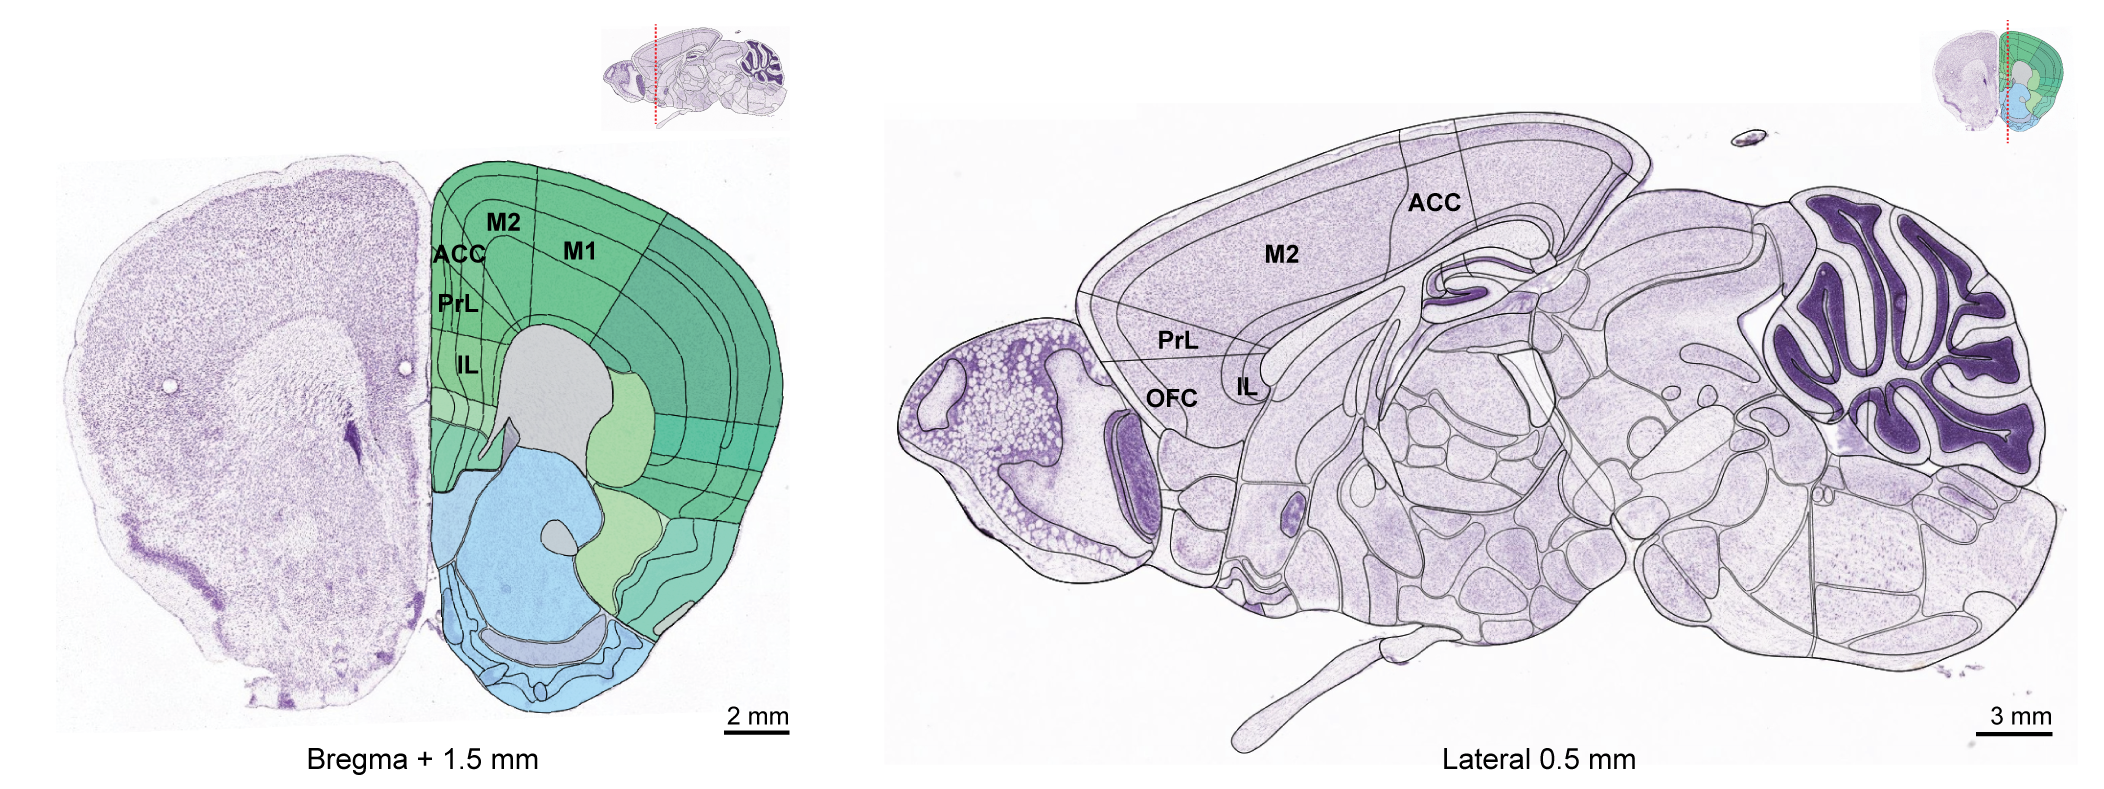
\includegraphics[width=\textwidth]{Figures/Introduction/Intro_fig_M2} 
\end{center}

\caption[Anatomical location of the secondary motor cortex]
{Anatomical location of the secondary motor cortex (M2) in the mouse. The images show an example Nissl-stained coronal (left) and saggital section (right) of the mouse brain containing M2, overlaid with approximate cytoarchitectural boundaries as defined in the Allen Mouse Brain Atlas. The anterior-posterior and medial-lateral coordinates of these sections are indicated by red dashed lines in the insets, and approximate the region of M2 imaged for the experiments in Chapters 1--3. Cortical areas in the coronal section are shaded in green. M1, primary motor cortex. ACC, anterior cingulate cortex including cingulate areas 1--2. PrL, prelimbic cortex. IL, infralimbic cortex. OFC, orbitofrontal cortex. All images were adapted from the Allen Mouse Brain Atlas (\url{https://mouse.brain-map.org/}.}

\label{fig:CC_fig1}
\end{figure}
